\documentclass[12pt, a4paper]{article}
\usepackage{amsmath,amsthm,amsfonts,amssymb,amscd}
\usepackage{graphicx}
\usepackage{multicol}
\usepackage{mathtools}
\usepackage[utf8]{inputenc}
\usepackage[brazil]{babel}
\usepackage{lettrine}
\usepackage{float}
\usepackage{caption}
\usepackage{subcaption}
\usepackage{algpseudocode}
\usepackage[sfdefault]{FiraSans} 
\usepackage{FiraMono}
\usepackage[T1]{fontenc}
\renewcommand*\oldstylenums[1]{{\firaoldstyle #1}}
\usepackage[cm]{sfmath}
\usepackage{setspace}
\usepackage[pdftex,plainpages=false,pdfpagelabels,pagebackref,colorlinks=true,citecolor=DarkGreen,linkcolor=NavyBlue,urlcolor=DarkRed,filecolor=green,bookmarksopen=true]{hyperref}
\usepackage[all]{hypcap}
\usepackage[round,sort]{natbib}
\usepackage{emptypage}
\fontsize{60}{62}\usefont{OT1}{cmr}{m}{n}{\selectfont}
\usepackage[T1]{fontenc}
\usepackage{indentfirst}
\usepackage{makeidx}
\usepackage[nottoc]{tocbibind}
\usepackage{type1cm}
\usepackage{listings}
\usepackage{titletoc}
\usepackage{pifont}
\usepackage[fixlanguage]{babelbib}
\usepackage[font=small,format=plain,labelfont=bf,textfont=it]{caption}
\usepackage[usenames,svgnames,dvipsnames]{xcolor}
\usepackage[a4paper,top=2.54cm,bottom=2.0cm,left=2.0cm,right=2.54cm]{geometry}
\usepackage{pdfpages}

\urlstyle{same}

\title{\textbf{Relatório Final de MAC0213 - Atividade Curricular em Comunidade}}
\author{
    \textbf{Aluno:} Luís Felipe de Melo Costa Silva \\
    \textbf{Número USP:} 9297961
    }
\date{}

\begin{document}
\maketitle

\section*{Introdução}

Este projeto foi fruto de uma parceria entre o Tecs - Grupo de computação social da USP e a Secretaria Municipal de Educação (SME) de São Paulo. Ele consiste em uma Análise Histórica dos Dados sobre o Atendimento das Creches de São Paulo, de junho de 2006 a dezembro de 2017. Este relatório segue o que está escrito no \href{https://lsflp.github.io/MAC0213/}{\textit{site}} oficial da disciplina, que complementa esse texto com mais detalhes.

\section{Tecnologias e Dados}

Para a realização do projeto, foram usadas algumas fontes de dados. Uma delas foram os dados educacionais, provenientes do \textit{site}\footnote{\url{http://dados.prefeitura.sp.gov.br/}} da prefeitura. Deles, apenas o recorte relacionado às creches (Matrículas e Demanda) foi utilizado.

Outra fonte foi a de dados populacionais, vindos do \textit{site}\footnote{\url{http://www.seade.gov.br/}} da Fundação SEADE. Desses dados, apenas a faixa etária de 0 a 3 anos foi utilizada. Junto com os dados educacionais selecionados, esses dados foram salvos num arquivo separado, utilizado para todas as análises.

Além desses dados, foram usados os dados das subdivisões de São Paulo em cinco zonas, de acordo com o Plano Diretor Estratégico de 2002 (PDE), também proveniente do \textit{site} da Prefeitura.

O desenvolvimento da análise foi inteiramente feito em Python 3\footnote{\url{https://www.python.org/}}. A ferramenta utilizada para os códigos foi a Jupyter\footnote{\url{http://jupyter.org/}}, que coloca o desenvolvimento numa janela de navegador Web. A principal biblioteca de análise utilizada foi a Pandas\footnote{\url{https://pandas.pydata.org/}}, que permite a conversão de dados .csv para estruturas de dados com usabilidade simples. Para os gráficos, foi usada a Matplotlib\footnote{\url{https://matplotlib.org/}}.

\section{Análises feitas}

As análises geraram um \href{https://lsflp.github.io/MAC0213/relatorios/relatorio.pdf}{relatório} final, que compila todas as descobertas feitas durante o semestre. Ele está disponível \textit{online}, e na íntegra.

\subsection{Análise Municipal}

A Análise Municipal juntou os dados dos distritos para obter os dados da cidade como um todo. Foi gerado um gráfico com a evolução da população total, das matrículas e da demanda, e, a partir disso, se tentou entender como tais variáveis se comportam. Se destaca a sazonalidade que acontece na fila e o crescimento quase que linear das matrículas. Também são vistas tabelas que comparam o primeiro e o último dados da amostra, assim como o primeiro e último mês de dezembro, para a demanda.

\subsection{Análise Distrital}

A Análise Distrital segue o mesmo padrão da Análise Municipal. A diferença é que a unidade de análise são os distritos. A maioria dos distritos segue o mesmo padrão identificado no município. Foi feita aqui uma análise para ver quantos distritos estão numa situação confortável, ou seja, com mais matrículas do que demandas. Essa análise é acompanhada de um apêndice que possui uma página com mais informações para cada distrito.

\subsection{Distribuição do Atendimento}

A terceira análise utiliza de mais recursos visuais para entender como o atendimento ocorre pelo município. São feitos mapas que analisam as matrículas e as demandas absolutas, as taxas de matrículas e demanda proporcionais à população. Também tem mapas que mostram a evolução do atendimento entre junho de 2006 e dezembro de 2017, para as matrículas e entre dezembro de 2006 e dezembro de 2017, para a demanda.

\subsection{\textit{Rankings}}

Os \textit{rankings} apresentam a classificação dos distritos em relação a quatro aspectos: matrículas absolutas, demanda absoluta, matrícula proporcional à população e demanda proporcional à população. Além disso, é feita uma comparação com um \textit{ranking} do primeiro período comparativo da amostra (junho de 2006 para as matrículas e dezembro de 2006 para a demanda, por conta da sazonalidade da fila). Esse segundo \textit{ranking} não está exibido no relatório final. O primeiro está anexo em um apêndice.  

\subsection{Análise de Tendências}

Aqui, tentou-se entender como se comportam três informações: o futuro das matrículas, o futuro das demandas e quando acontece uma inversão a favor das matrículas, ou seja, um distrito possui mais matrículas do que demanda. Para cada uma dessas informações existe um \textbf{ranking}, presente num apêndice do relatório.

\section{Conclusão da Análise}

A partir da análise dos dados, foi possível tirar algumas conclusões. Pôde-se ver que o município melhorou como um todo. Também se nota que ele está no caminho certo, com as matrículas aumentando e a fila diminuindo. No entanto, ainda faltam mais matrículas para que ele atinja a meta proporcional de 75\%.

A evolução do atendimento foi diferente pelos distritos. Quase todos apresentaram aumento nas matrículas, uns mais do que outros, como o distrito de Lajeado, que subiu 14 posições no \textit{ranking} de matrículas absolutas e 62 no \textit{ranking} de matrículas proporcionais à população. Em contrapartida, o distrito da República foi o único que apresentou queda nas matrículas.

Pensando nas filas, é possível confirmar que elas caíram na maioria dos distritos. No entanto, alguns distritos apresentaram aumento, como a Vila Andrade, Pedreira e Marsilac.

O distrito do Marsilac, o mais meridional da cidade, é o único que atende mais de 100\% de sua população estimada. Tal informação leva a uma reflexão quanto a acurácia das estimativas populacionais e também em relação a distritos que atendem crianças de outro distrito, este último um fato que não pode ser ignorado ao longo da leitura dessa análise.

De acordo com os dados mais recentes, os distritos que apresentam o maior número de vagas se localizam na periferia das zonas Sul, Leste e Norte. São as mesmas regiões que concentram boa parte da demanda. Contudo, foram justamente essas regiões que tiveram os maiores aumentos no número de matrículas e maiores reduções na fila.

Portanto, conclui-se que, embora o município de São Paulo esteja melhorando no atendimento de creches, essa melhora não é refletida de maneira igual pela cidade. Isso não deve ser considerado um fato ruim, e se deve a diversas razões. Uma delas é que a população se distribui de maneira diferente pela cidade e outra é que nem todas as crianças se matriculam em creches municipais, frequentando a rede privada. Acontece também de crianças com idades entre 0 e 3 anos não estarem matriculadas em nenhum lugar, ficando em casa, com parentes, por exemplo.

\section{Arquivos construídos}

Para fazer as 5 análises supracitadas, foram gerados 10 arquivos em Python 3, cada um com uma parte da análise.

\begin{enumerate}
	\item \textbf{Filtro de arquivos}: Sua ideia era de pegar os arquivos de dados obtidos das fontes externas, limpar o que não seria usado durante o semestre, arrumar parte dos dados e então, salvar o produto em um arquivo resultante que seria usado em todos os outros \textit{notebooks}. Contribui com \textbf{todas} as análises.
	\item \textbf{Gráficos de tempo}: Gera um gráfico de evolução da população, das matrículas e da demanda para cada um dos 96 distritos da cidade de São Paulo, a partir dos dados filtrados. Um exemplo de seu produto pode ser visto na \autoref{fig:temposantana}. Esse arquivo ajudou na elaboração da \textbf{Análise Distrital} e da \textbf{Análise Municipal}, pelo conhecimento obtido.
	\begin{figure}[H]
		\centering
		\includegraphics[width=0.7\linewidth]{../Analises/graficos/tempo/tempo_SANTANA}
		\caption{Evolução das matrículas, da demanda, e da população de 0 a 3 anos no distrito Santana.}
		\label{fig:temposantana}
	\end{figure}
	\item \textbf{Mapas}: Esse \textit{notebook} serve para gerar os mapas de distribuição das matrículas e da demanda pela cidade. Foi o que levou mais tempo para ficar pronto, em torno de 10 dias. Um de seus resultados pode ser visto na \autoref{fig:evabspccreche}. Ele contribuiu com o desenvolvimento da análise de \textbf{Distribuição do Atendimento}.
	\begin{figure}[H]
		\centering
		\includegraphics[width=0.5\linewidth]{../Analises/mapas/MAT_CRECHE_jun-06}
		\caption{Mapa que mostra o número de matrículas pela cidade em junho de 2006, primeiro dado da amostra.}
		\label{fig:evabspccreche}
	\end{figure}
	\item \textbf{Análise Municipal}: Cuida de transformar (no caso, somar) todos os dados referentes ao município (total populacional estimado de 0 a 3 anos, número de matrículas e demanda) para posterior análise. Ajuda na \textbf{Análise Municipal}, como pode-se pensar. Também gera um gráfico como o da \autoref{fig:evabspccreche}.
	\item \textbf{Agrupamentos}: A ideia de criar esse arquivo era para gerar gráficos de dispersão que mostrariam como os distritos podem ser agrupados, no entanto, após algumas experiências, foi observado que os distritos sempre estão relativamente próximos, em taxas de atendimento relativas. Gráficos feitos aqui podem ser visto na análise de \textbf{Distribuição do Atendimento}.
	\item \textbf{Comparação}: Esse \textit{notebook} serviu para comparar cada distrito com o município. Foram feitos gráficos que mostram a evolução da participação proporcional de cada distrito no município (um deles pode ser visto no \href{https://lsflp.github.io/MAC0213/poster/poster_a1.pdf}{\textit{pôster}} feito para a disciplina) e gráficos que exibem a evolução do distrito no \textit{ranking} municipal (esses últimos nunca usados, porém essenciais para a ideia da análise de \textbf{\textit{Rankings}}).
	\item \textbf{Listas}: Constrói dois gráficos apenas: um que mostra o número de matrículas em junho de 2006 nos distritos sobreposto às matrículas em dezembro de 2007 e um outro que compara a demanda em dezembro de 2006 com a demanda em dezembro de 2007. O primeiro foi utilizado no \href{https://lsflp.github.io/MAC0213/poster/poster_a1.pdf}{\textit{pôster}} feito para a disciplina e o outro está presente numa versão \href{https://lsflp.github.io/MAC0213/poster/poster_a0.pdf}{\textit{alternativa}} do pôster. O conhecimento obtido aqui foi utilizado para a análise de \textbf{\textit{Rankings}}.
	\item \textbf{Previsão da demanda}: Usando um modelo conhecido como ARIMA\footnote{\url{https://pt.wikipedia.org/wiki/ARIMA}}, foi construída uma previsão de como a demanda vai se comportar num futuro próximo, a partir dos dados de entrada. Com isso, foi feito uma estimativa que mostra quando a demanda atingirá o valor zero. Usada na \textbf{Análise de Tendências}.
	\item \textbf{Previsão das matrículas}: Funciona do mesmo modo que o \textit{notebook} anterior. Sua variação se deve pelo fato de ele ser feito para a previsão das matrículas. A meta aqui não é atingir um valor absoluto, porque os distritos não têm as mesmas populações. Por isso, foi usado um valor proporcional de 75\%. Como não existem dados de estimativas populacionais para anos depois de 2018, foi usada a média populacional entre 1995 e 2017 como parâmetro de comparação. Mais detalhes estão na \textbf{Análise de Tendências}.
	\item \textbf{Inversões}: Procura quando ocorreu a última inversão entre demandas e matrículas, que é quando o número de matrículas fica maior que a demanda. Assume-se que uma posição confortável para um distrito seja quando ele possui mais matrículas do que demandas. Um total de 63 distritos possuíam mais fila do que matrículas em junho de 2006. Já em dezembro de 2017, apenas a Sé encontrava-se nessa condição. Para a \textbf{Análise de Tendências}, foi gerada uma tabela que mostra quando as inversões aconteceram pelos distritos.
\end{enumerate}

Também foram feitos alguns \textit{notebooks} auxiliares para a produção de texto automatizado para o Relatório Final entregue à SME.

\section{Relação com a SME}

A pessoa da SME com quem mais tive contato era a minha supervisora, Priscilla Corrêa, Assessora Técnica na Secretaria Municipal de Educação de São Paulo. Também tive contato com a Ananda Grinkraut, Analista de Políticas Públicas e Gestão Governamental. Nossa relação era pautada por conversas por e-mail e por mensagens. Uma foto nossa pode ser vista na \autoref{fig:img6634}

Fizemos algumas reuniões presenciais, a maioria delas na sede do Pátio Digital, na casa Sérgio Buarque de Holanda, recentemente reformada, localizada no Pacaembu, na zona Oeste da cidade. Uma outra reunião foi feita na sede da SME, na Vila Clementino, zona Sul da cidade.

\begin{figure}[H]
	\centering
	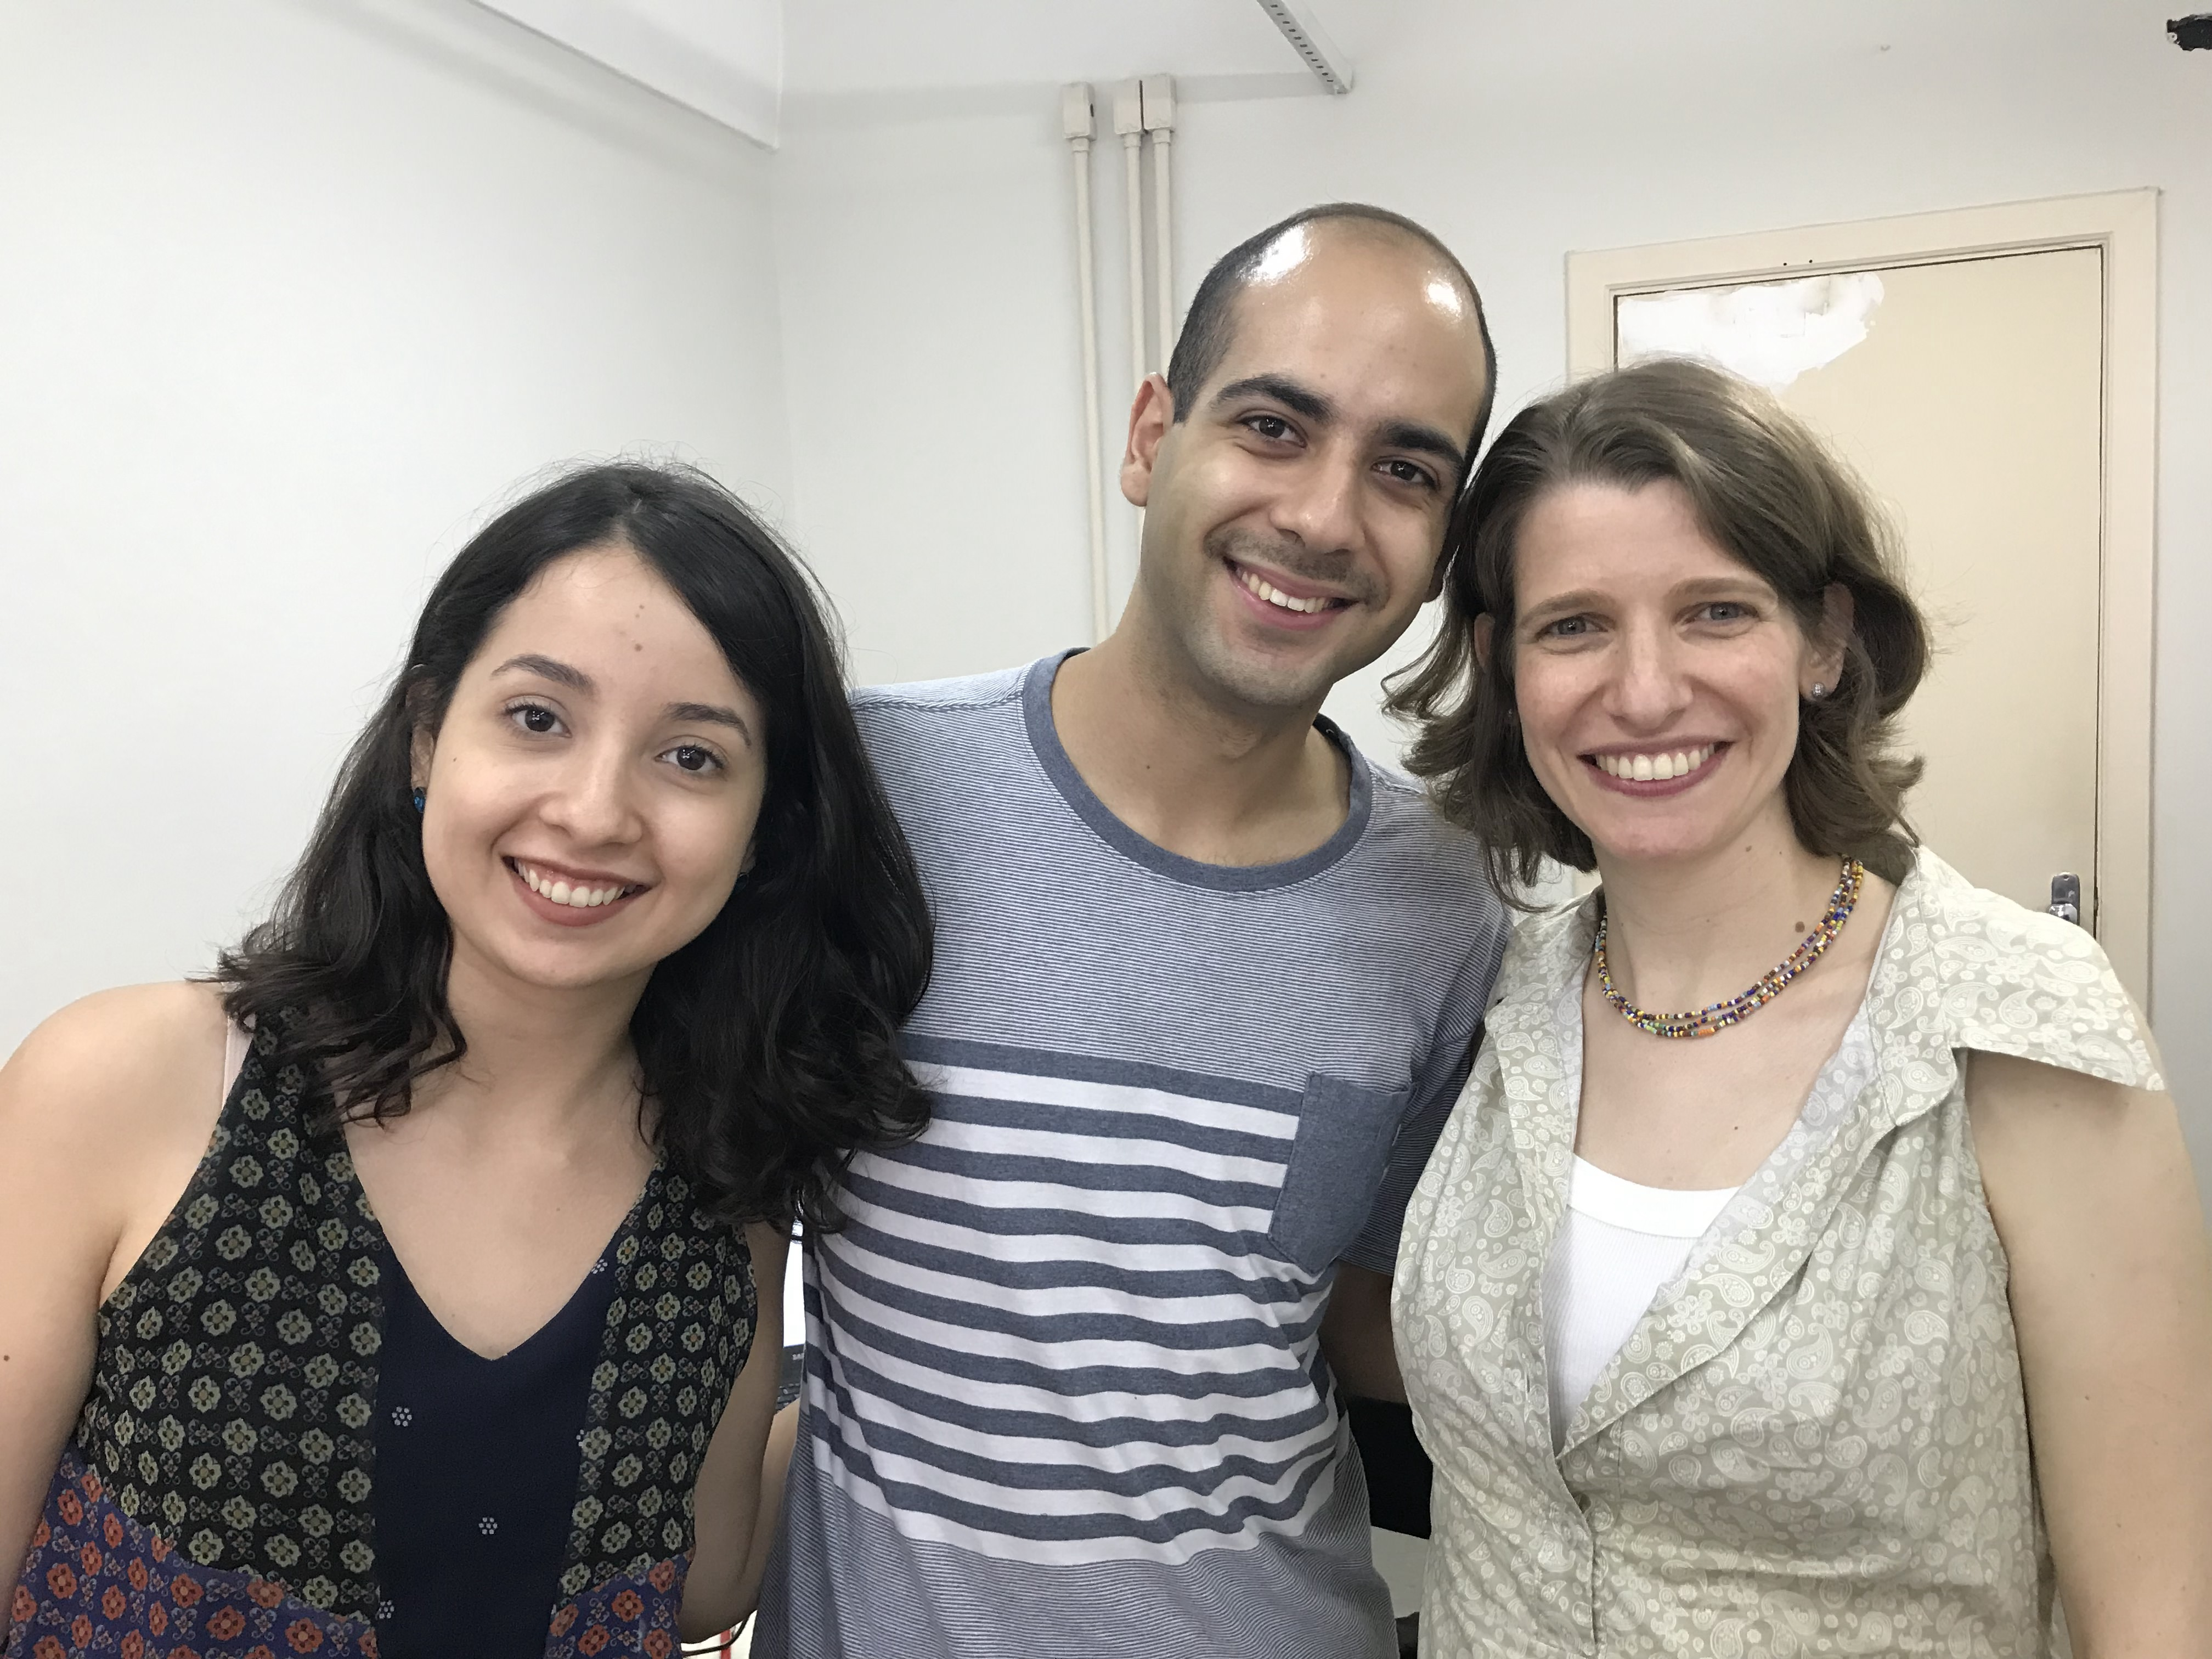
\includegraphics[width=0.7\linewidth]{IMG_6634}
	\caption{Da esquerda para a direita, Priscilla, eu e Ananda.}
	\label{fig:img6634}
\end{figure}


\section{Horas trabalhadas}

Para esta disciplina foi usado um total de \textbf{109 horas}, divididas como na tabela abaixo:

\begin{table}[H]
	\centering
	\begin{tabular}{l|l}
		\textbf{Atividade}                                   & \textbf{Horas Registradas} \\ \hline
		\textit{Reuniões e Apresentações com a SME} & 9                          \\ \hline
		\textit{Análises}                           & 77                         \\ \hline
		\textit{Elaboração do Relatório Final}    & 23                         \\ 
	\end{tabular}
\end{table}

A relação hora-mês pode ser vista na tabela a seguir:

\begin{table}[H]
	\centering
	\begin{tabular}{l|l}
		\textbf{Atividade}                                   & \textbf{Horas Registradas} \\ \hline
		\textit{Agosto e Setembro} & 25                          \\ \hline
		\textit{Outubro}                           & 40                         \\ \hline
		\textit{Novembro}    & 44                         \\ 
	\end{tabular}
\end{table}

Não estão incluídos nesses registros os tempos de elaboração do pôster da disciplina e da produção desse relatório. Também foram excluídos os tempos de comunicação com a SME (por e-mail e por mensagem) e tempos de deslocamento para as reuniões. 

Mais detalhes podem ser vistos na página de \href{https://lsflp.github.io/MAC0213/estatisticas.html}{estatísticas} do \textit{site} da disciplina.

Na página a seguir, está a confirmação das 100 horas trabalhadas.

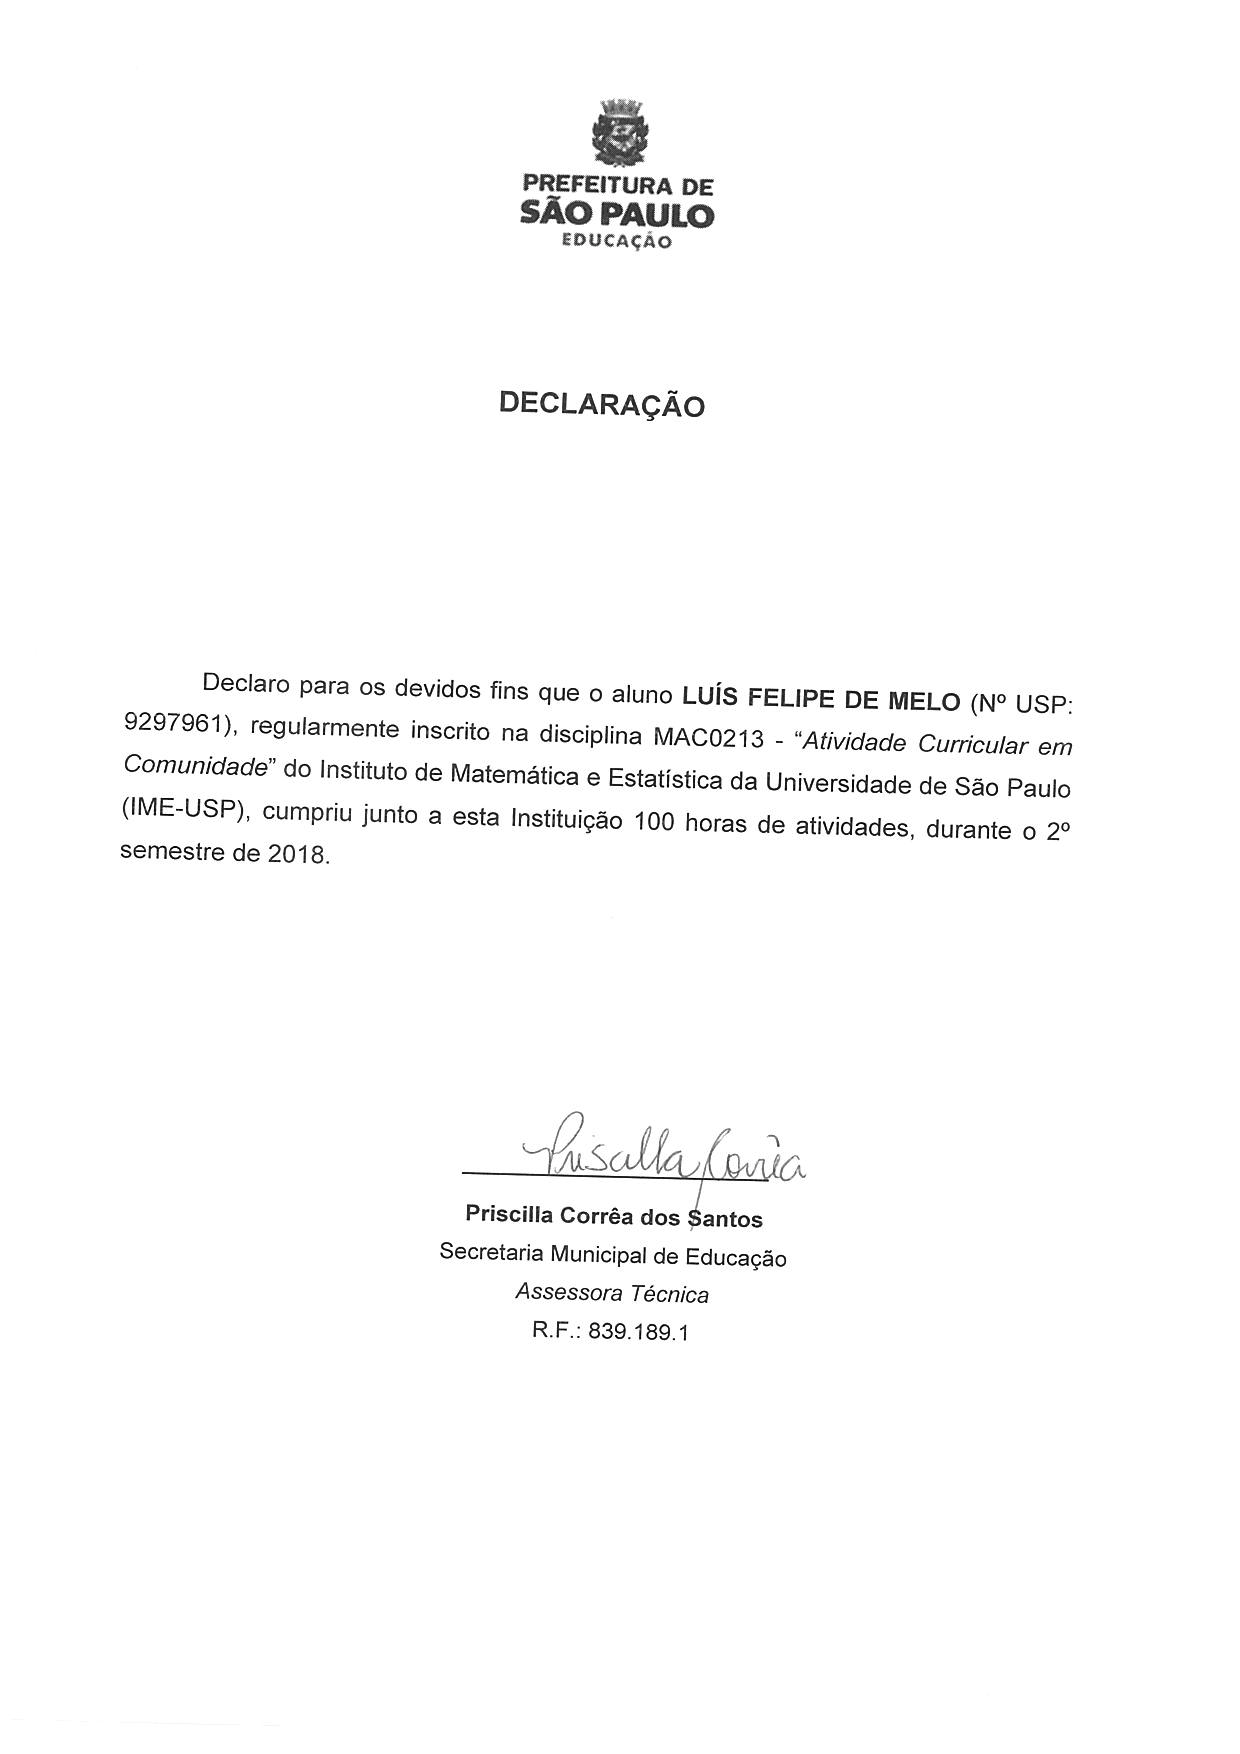
\includepdf{declaracao.pdf}

\section{Parte Subjetiva e Projetos Futuros}

Na minha opinião, o projeto foi muito enriquecedor. Foi a primeira vez que fiz um projeto grande de análise de dados. Não tive muita facilidade no começo, mas depois tudo começou a fazer mais sentido.

Foi a primeira vez que tive algum contato com um órgão governamental. A concepção muda bastante ao conhecer o trabalho que é feito por eles ao invés de só ouvir as notícias, que costumam destacar fatos negativos.

Para essa matéria precisei de muita organização. O primeiro motivo para isso é que os resultados seriam entregues apenas no fim do semestre. Quando vi que a média de horas que eu dedicava à disciplina estava aquém do necessário para cumprir as 100 horas mínimas, tive que estabelecer uma rotina de trabalhar para as análises pelo em torno de 90 minutos por dia. É possível observar que isso funcionou. 

As análises feitas aqui foram bem simples, e, no final, não precisaram de tanto conhecimento técnico. Para as próximas análises nesse tema, pode ser estudado quem são as crianças que frequentam as creches municipais, traçando um perfil sócioeconômico dos estudantes. Também é possível analisar quais são os critérios que mais influenciam na escolha das creches municipais. Algumas variáveis podem ser pequisadas, tais como oferta de vagas no distrito e renda das famílias. É possível também procurar agrupamentos entre os distritos, para caracterizá-los e traçar ações em comum para os grupos eventualmente identificados. 

\end{document}
